\section{Fitting Data}

\begin{slide}{Fitting Strategies}

  \begin{cenpage}{135mm}
  Data analysis seeks a {\RedEmph{Model}} that best matches a
  {\BlueEmph{Measurement}}.

  \vmm

  We'll use $\chi^2$ (don't confuse with EXAFS $\chi$!!) to describe how
  good the match is:

  \[ \chi^2  =
  \sum_i^{N_{\rm fit}} \frac{[\chi_i^{\rm measured} - \chi_i^{\rm
      model}({x})]^2}{\epsilon^2}
  \]

  where
  \begin{itemize}
  \item $N_{\rm fit} = $ number of points in the data to fit.
  \item $\epsilon = $ the  estimated noise  level in the data.
  \item $x$  is the set of parameters to be varied in the analysis
  \end{itemize}

  \begin{center}
    {\RedEmph{ The Best Fit is the one with lowest $\chi^2$. }}
  \end{center}

  \vmm   \hrule \vmm

  \onslide+<2->

  Questions:

  \begin{enumerate}
  \item How do I know how many independent measurements I have?
  \item What is $\epsilon$ for my data?
  \item What parameters can/should I vary?
  \end{enumerate}
\end{cenpage}
\end{slide}

\begin{slide}{The Information Content of EXAFS}

\begin{cenpage}{135mm}
    The number of parameters we can reliably extract from our data is limited:
    \vspace{1mm}


    \begin{postitbox}{26mm}
      $\displaystyle  N_{\rm idp} \approx { \frac{2 \Delta k \Delta R}{\pi}}  $
    \end{postitbox}

    \vmm

    where $\Red{ \Delta k}$ and $\Red{ \Delta R}$ are the $k$- and
    $R$-ranges of the usable data.

    \onslide+<2->
    \vmm\vmm

    For a typical range of $k = [3.0, 12.5] \rm\,\AA^{-1}$ and $R = [1.0,
    3.0] \rm\,\AA$, there are $\sim 12$ parameters that can be determined
    from EXAFS.      \onslide+<2-> That's not much!

    \onslide+<2->
    \vmm\vmm

    The Fit statistics and confidence in the measured parameters need to
    reflect this.  But we usually oversample our data ($N_{\rm fit} >
    N_{\rm idp} $) so we have

    \begin{postitbox}{56mm}
      $ \displaystyle
      \chi^2  =  \frac{ N_{\rm idp}}{\epsilon^2 N_{\rm fit}}
      \sum_i^{N_{\rm fit}} [\chi_i^{\rm measured} - \chi_i^{\rm model}({x})]^2
      $
    \end{postitbox}

    Note: I also assumed $\epsilon$ is a constant.

\vfill
\end{cenpage}
\end{slide}


\begin{slide}{Other Fitting Statistics}

  \begin{cenpage}{135mm}
  Other ``goodness-of-fit statistics'':
  \vmm

  {\RedEmph{chi-square}}: As before:

  \begin{postitbox}{54mm}  $ \displaystyle
    \chi^2  =  \frac{ N_{\rm idp}}{\epsilon^2 N_{\rm fit}}
    \sum_i^{N_{\rm fit}} [\chi_i^{\rm measured} - \chi_i^{\rm model}({x})]^2
    $
  \end{postitbox}

 \vmm
  {\RedEmph{reduced chi-square}}: scale $N_{\rm varys}$ by the ``degrees of freedom'' :

  \begin{postitbox}{38mm}
    $ \chi^2_\nu =  \chi^2 / (N_{\rm idp}-N_{\rm varys}) $
  \end{postitbox}


  For a ``Good Fit'', $\chi^2_\nu$ should be $\sim$ 1.   This
  {\RedEmph{never}} happens!

\vmm

  {\RedEmph{R-factor}}: $\cal{R}$  gives a ``fractional misfit'' (and
  not scaled by the data  uncertainty $\epsilon$):

\vmm

  \begin{postitbox}{50mm}
    \[
{\cal{R}} = \frac{\sum_i^{N_{\rm fit}}[\chi_i^{\rm measured} -
      \chi_i^{\rm model}({x})]^2 }{
      \sum_i^{N_{\rm fit}} [{\chi_i^{\rm measured}}]^2}
    \]
  \end{postitbox}

\vfill
\end{cenpage}
\end{slide}

%%%%%%%%%%%%%%%%%%%%%%


\section{Uncertainties in $\chi(k)$}
\begin{frame}\frametitle{Propagation of uncertainties in $\chi(k)$}

\begin{cenpage}{135mm}

  Estimating uncertainties in  $\chi(k)$ has always been a challenge.

  \vmm

  We have (by default) estimated the uncertainty in $\chi(k)$ as
  {\BlueEmph{white noise}} {\tiny{(Newville, Boyanov, and Sayers, {\emph{J
          Synch Rad}}, 1999)}}, using $\chi(R)$ between [15, 25] \AA.

\begin{columns}
  \begin{column}[T]{60mm}

    {\onslide+<1->  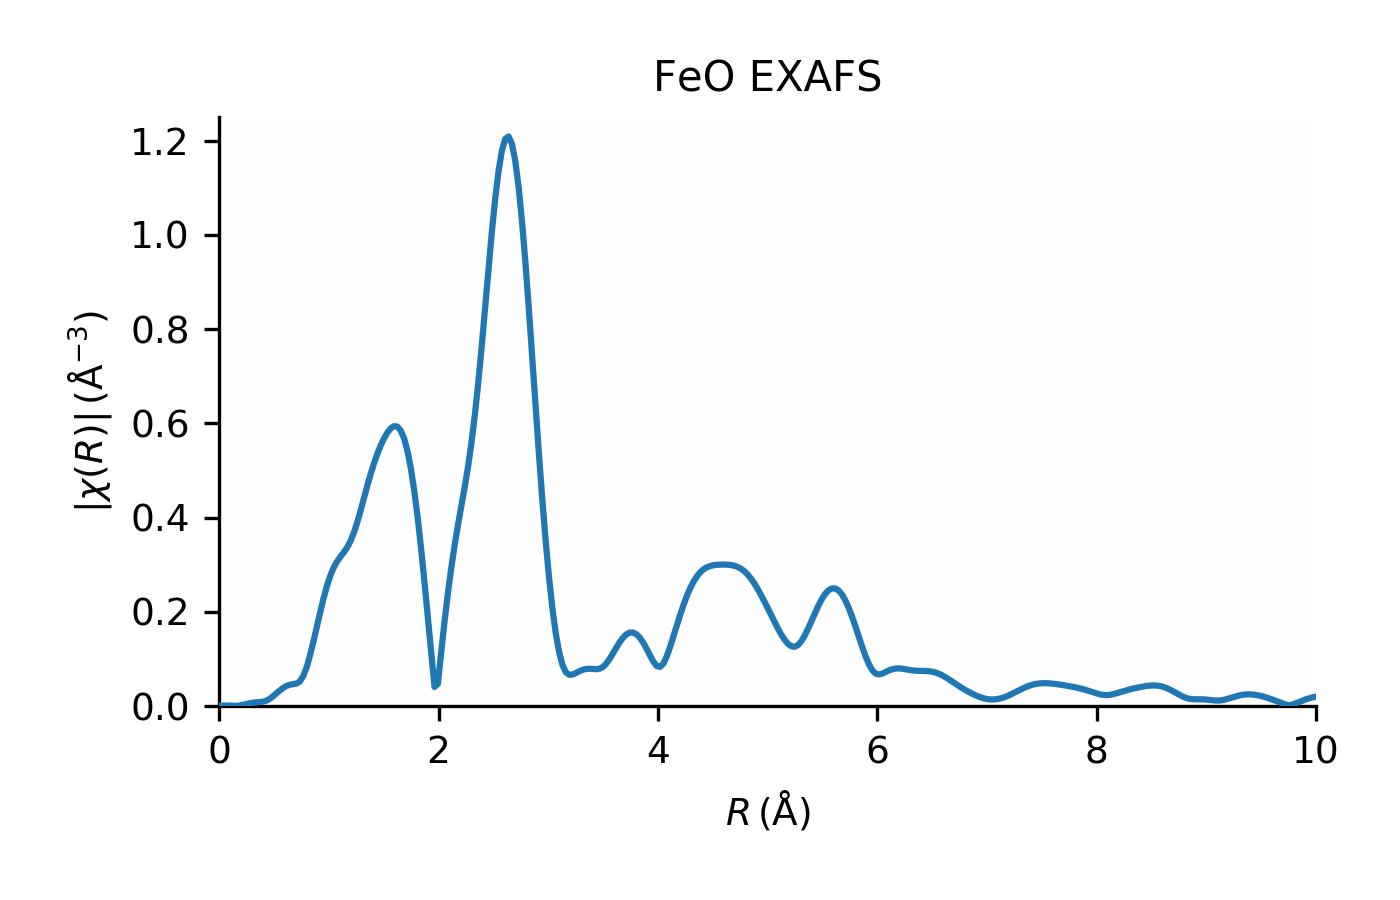
\includegraphics[width=60mm]{figs/errors/feo_chir}  }


  \end{column}
  \begin{column}[T]{60mm}

    {\onslide+<2-> 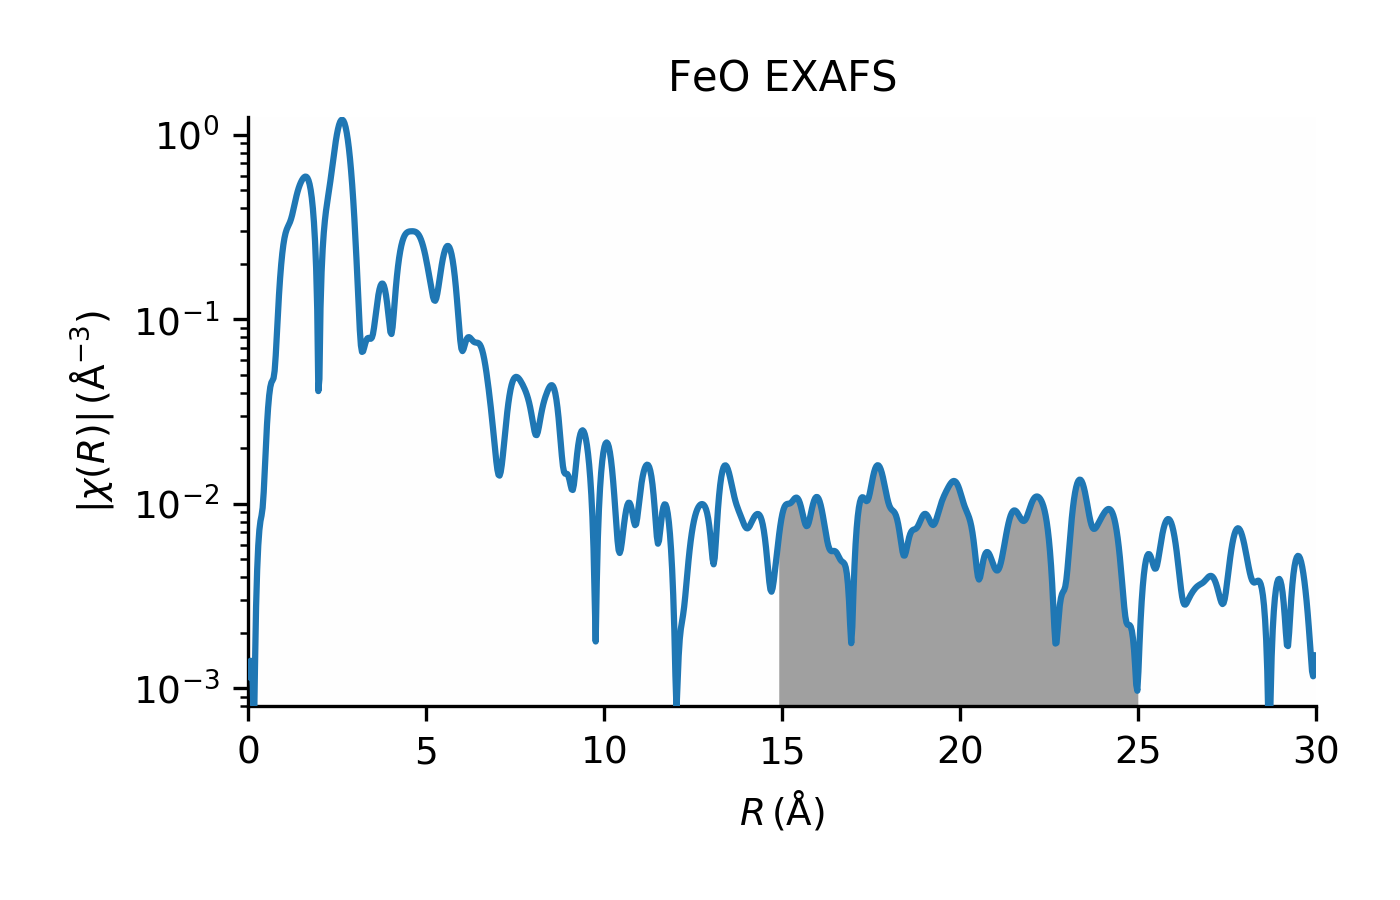
\includegraphics[width=60mm]{figs/errors/feo_chir_logscale} }

  \end{column}
\end{columns}

{\onslide+<2->

  \begin{cenpage}{105mm}


    The ``high-R'' portion of $\chi(R)$ can estimate the
    ``white noise'' in the data pretty well.

    \vmm
    This is easy to do, but we know it misses an important component:
  \end{cenpage}


  \begin{postitbox}{63mm}
      {uncertainties from  background subtraction}
  \end{postitbox}

}
\end{cenpage}

\end{frame}


\begin{frame}\frametitle{ Uncertainties in $\chi(k)$ from background subtraction}

  \begin{cenpage}{135mm}

\vmm
\begin{cenpage}{105mm}

  We can propagate the uncertainties from the fit of the background spline
  to estimate the uncertainty in $\chi(k)$ from the background subtraction.

  \vmm \vmm

  This is {\BlueEmph{not white noise}}.   In fact, it tends to have a peak
  somewhat above $2 R_{\rm bkg}$
\end{cenpage}

\begin{columns}
  \begin{column}[T]{60mm}

    {\only<1> { 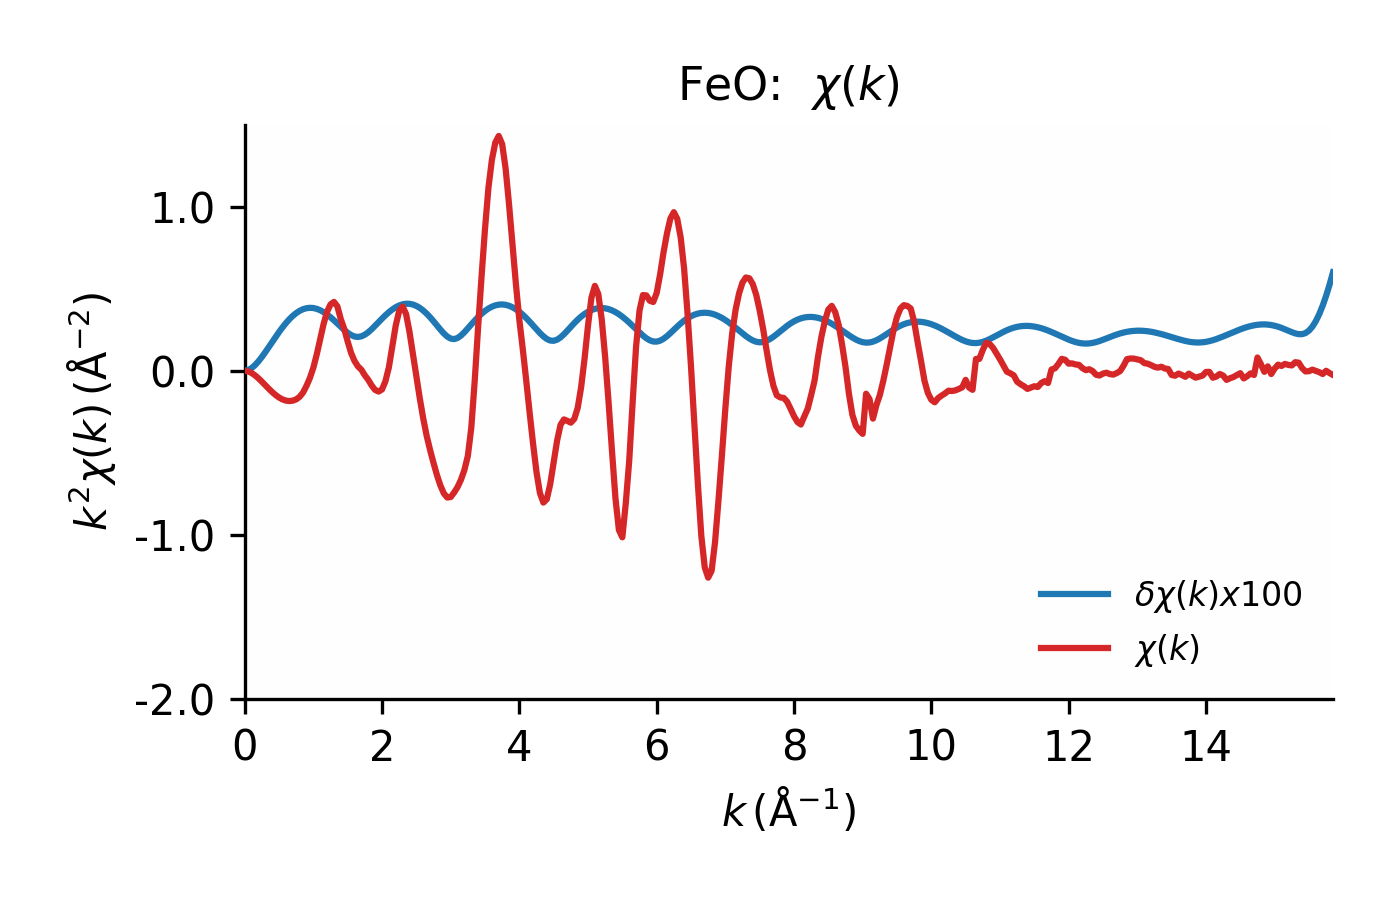
\includegraphics[width=60mm]{figs/errors/feo_chik_deltachi}}}

    {\only<2,3> { 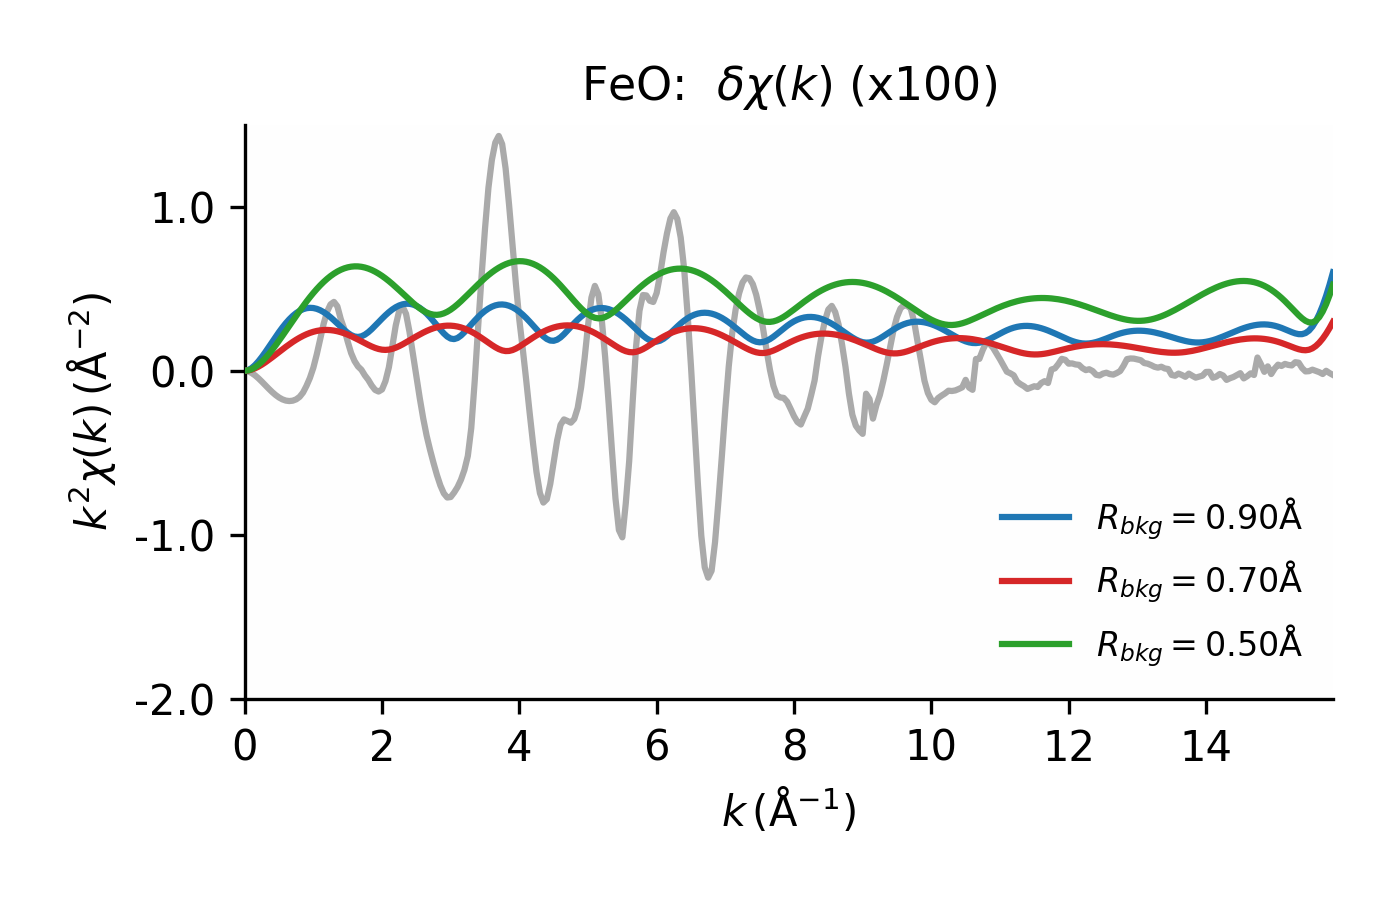
\includegraphics[width=60mm]{figs/errors/feo_deltachik_rbkg} }}

    \end{column}

    \begin{column}[T]{60mm}

      {\only<1>{ 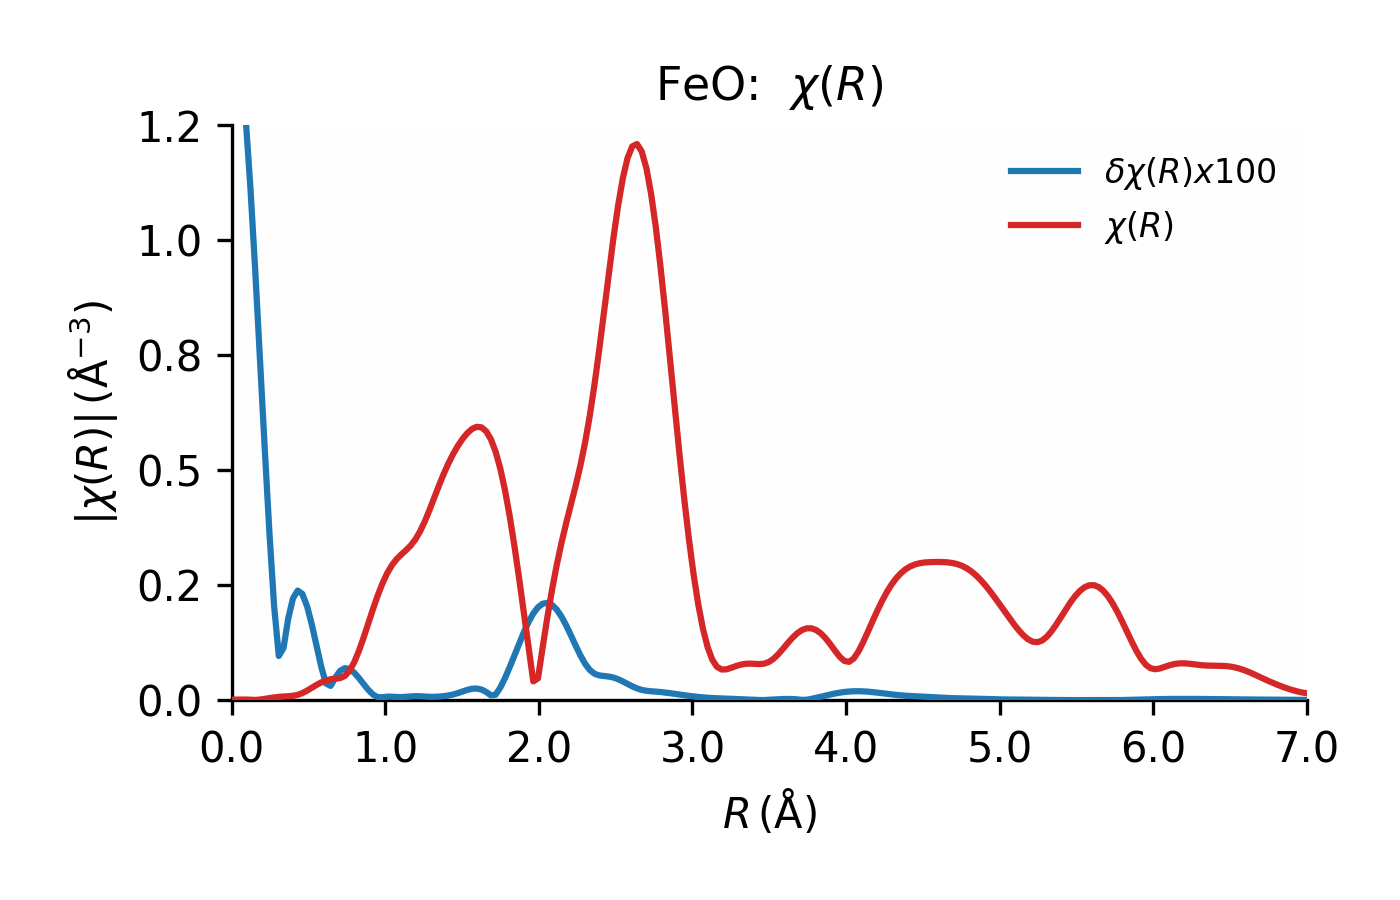
\includegraphics[width=60mm]{figs/errors/feo_chir_deltachi} }}

      {\only<2,3>{ 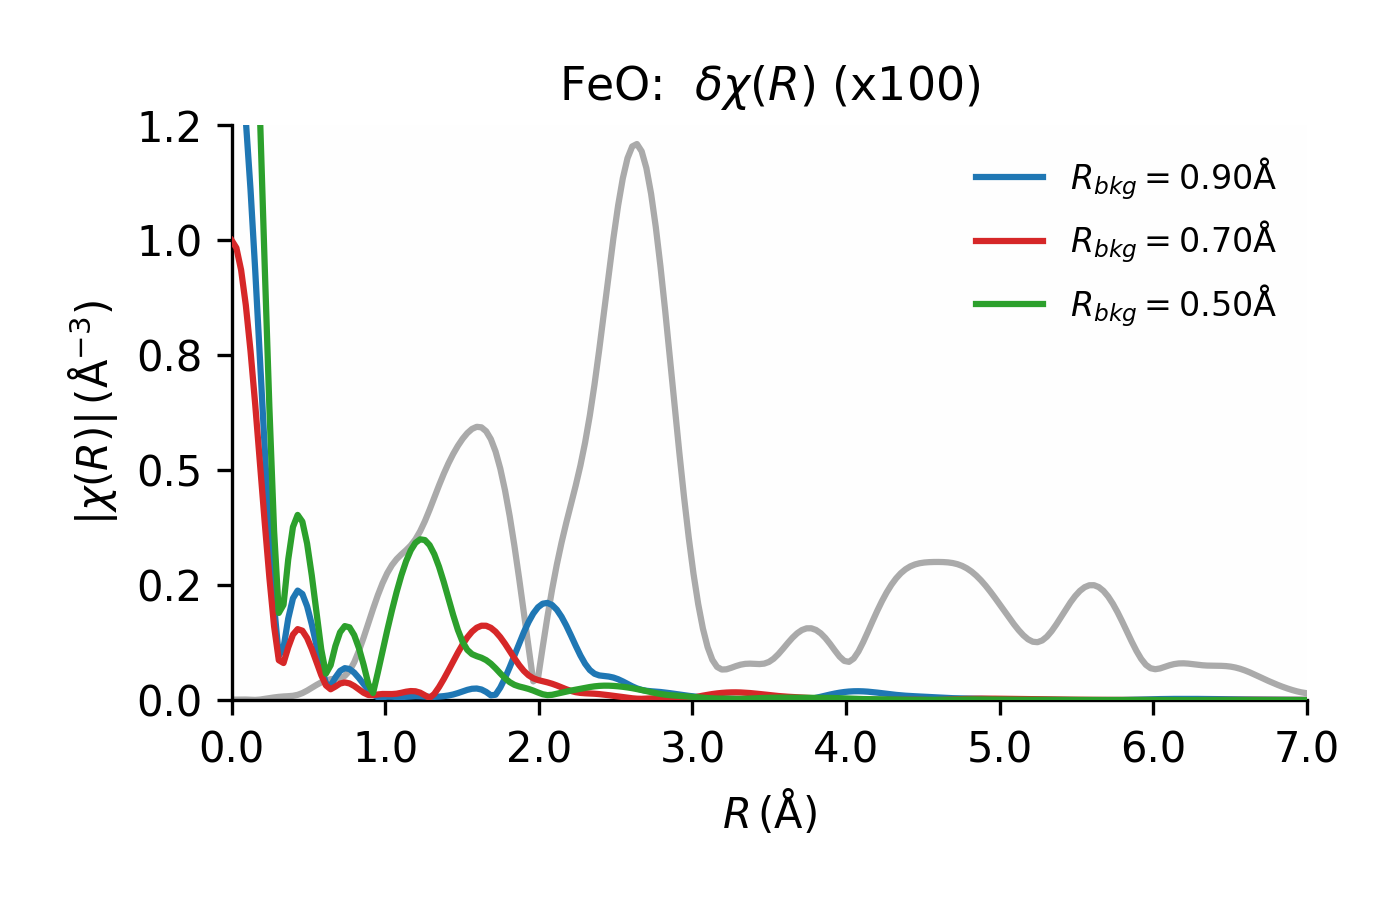
\includegraphics[width=60mm]{figs/errors/feo_deltachir_rbkg} }}

    \end{column}

\end{columns}

\vmm

{\onslide+<3-> {

\begin{cenpage}{105mm}

    Using this $\delta\chi(k)$ array reduces the $\chi^2$
    statistic by $2\times$ or  more.

\end{cenpage}

}}

\end{cenpage}
\end{frame}

%%%%%%%%%%%%%%%%%%%%%%
\begin{slide}{Error Bars: the uncertainties in the fit variables}

\begin{cenpage}{125mm}
A fit finds a set of values $\Blue{x_0}$ that are the ``best fit'' of the variables
$\Blue{x}$ -- they give the lowest value of  $\chi^2$.

\begin{center} Uncertainties in $\Blue{x}$ are estimated by increasing the
  $\chi^2$ by 1: \end{center}


\begin{columns}
\begin{column}{58mm}

\onslide+<2->

 \wpdf{58mm}{figs/errors/ellipse}

\end{column}
\begin{column}{55mm}

{\onslide+<2->
Some Parameters are {\RedEmph{Correlated}}:

\vmm

Changing {\Blue{$x$}} away from its best value will change the best value
for {\Blue{$y$}}.

\vmm

\begin{postitbox}{53mm}
  For EXAFS, ($R$, $E_0$) and ($N$, $\sigma^2$) are usually very highly
  correlated ($>0.85$).
\end{postitbox}
\vmm
}
\end{column}
\end{columns}

 \onslide+<2-> \vmm
 {\RedEmph{Increasing $\chi^2$ by 1 assumes we have a ``Good Fit'', with $\chi^2_\nu \approx 1$}}.

 \vmm We typically have  $\chi^2_\nu \gtrsim 50$  (Actually, we  {\emph{can
     now do better}}!).

\vmm
We increase the best $\chi^2$ by $\chi^2_\nu$ to estimate error bars.


\vmm \vmm
\end{cenpage}

\end{slide}

% %%%%%%%%%%%%%%%%%%%%%%
% \begin{slide}{Error Bars: correlations between fit variables}


%     Pairs of variables can be {\RedEmph{correlated}}: changing one variable away
%     from its optimum value can be compensated by changing another variable away
%     from its best value.  The uncertainties needs to take correlations into
%     account.

%     \vmm\pause

%     \begin{center} \wpdf{50mm}{figs/errors/ellipse2}   \end{center}

%     \vmm
%     The uncertainty in $x$ is $\delta x$, NOT  $\delta x'$!

%     \vmm

%     The correlation between variables is given by the slope of the ellipse:

%     \begin{postitbox}{75mm}    how much does $y$ want to change when
%       changing $x$?
%     \end{postitbox}

%     \vmm

% \vfill
% \end{slide}
